\subsubsection{Fault Model Paradigms}
\label{ssec:fault}

\begin{figure}
\begin{center}
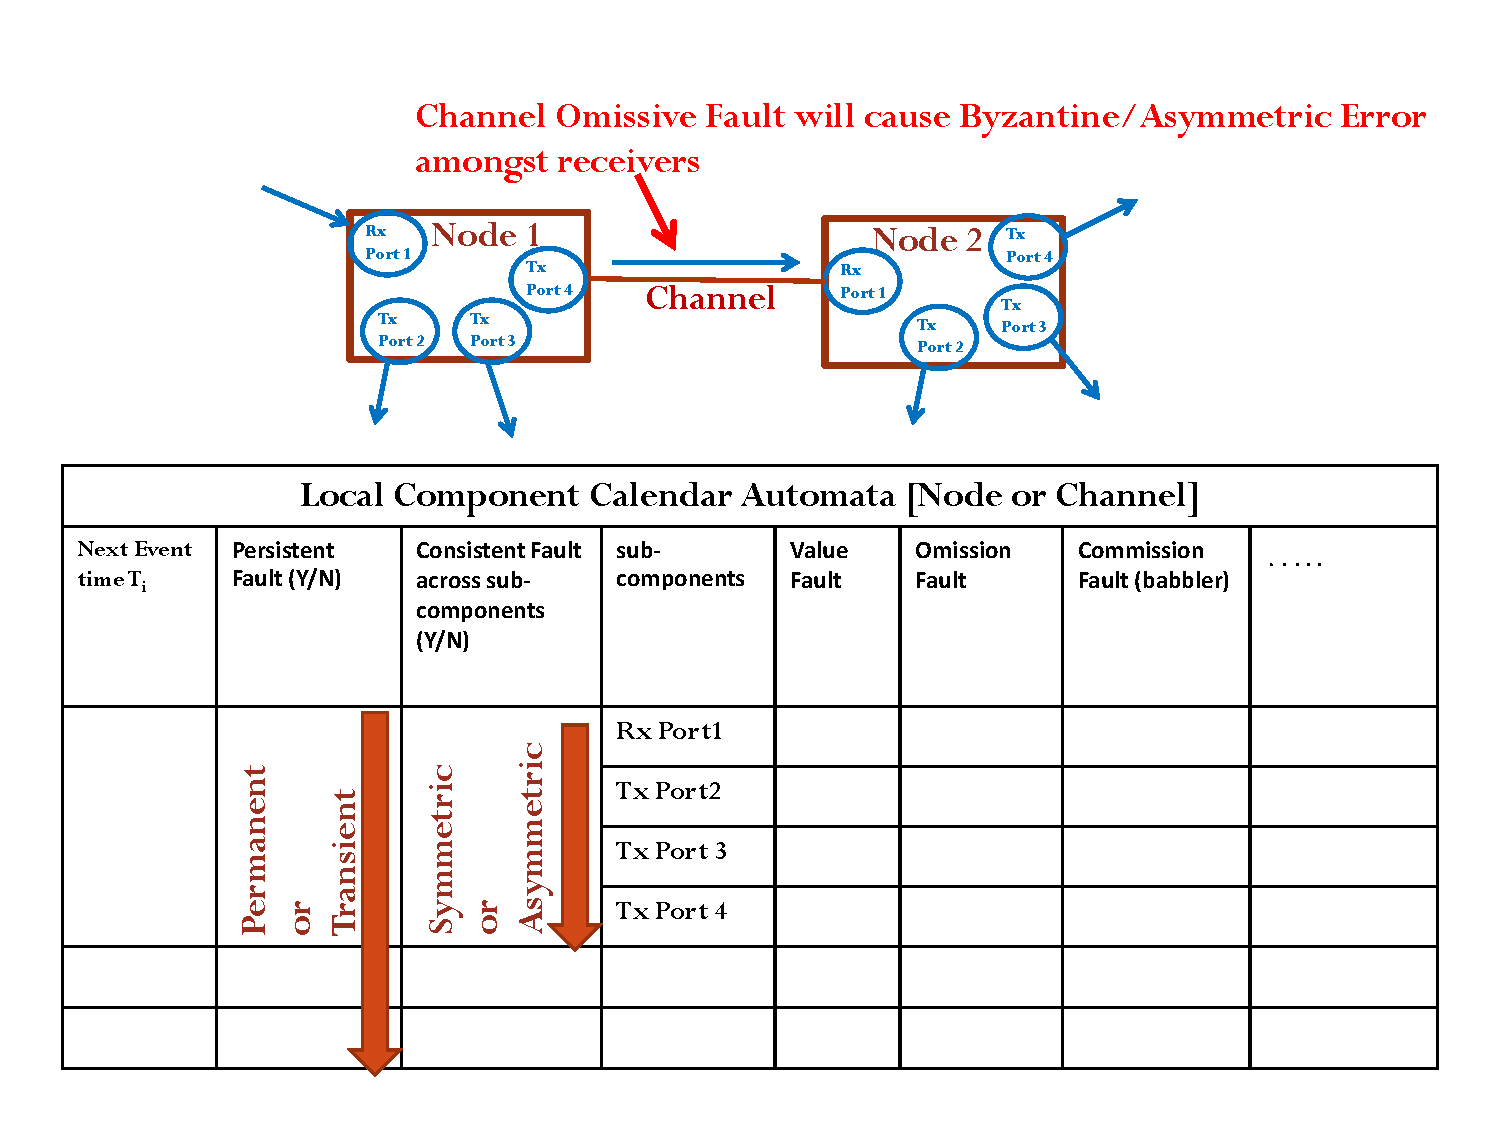
\includegraphics[width=0.7\textwidth]{figures/local_faults.pdf}
\caption{Local Component Fault Models}
\label{fig:local_faults}
\end{center}
\end{figure}

Our fault model is the most inchoate of the primitives developed in the
ADSL. Following the taxonomy of Avizienis~\emph{et~al.}~\cite{taxonomy}, we
refer to faults that occur locally in any component like a node of channel in
networked system as being modeled as \emph{local faults}. Some examples of local
faults are:
\begin{itemize}
  \item Omission (message loss)
  \item Commission (babbling)
  \item Untimely (late, early, sequence violation etc.)
  \item Invalid value (semantic, syntactic,..)
  \item Invalid protocol behavior (e.g., failure of fault handling of detection, protection etc).
\end{itemize}

On the other hand, \emph{global faults} are based on relationships between two
or more components (nodes/channels) at the system level. Examples of system
faults include symmetric and asymmetric transmission faults. Global faults may
be dependent on the expectation of degree of consensus, which in itself is tied
to the application's sensitiveness to disagreements, independence assumptions,
or degree of maliciousness (e.g. assumptions on how coordinated two or more
nodes can be in triggering failures).

As discussed in Section~\ref{sec:adsl}, we use a calendar
automata abstraction to manage global time keeping across a system model system
in order to manage synchronous and asynchronous clock models. Hence, we propose
managing both local and global faults also via calendar too. For example, in
Figure~\ref{fig:local_faults}, we show a small sub-network of larger network
where there are two nodes, $Node_1$ and $Node_2$ connected by a channel. The two
nodes are intermediate relays whereby $Node_1$ receives message on receive
$Port_1$ and broadcasts to all its output transmit ports. Similarly, $Node_2$
receives messages from $Node_1$'s transmit port four on the channel into its own
receive port one, and subsequently, it also broadcasts on all its output
ports.

An omissive fault on the channel component will cause
Byzantine/asymmetric faults to occur because receivers connected to $Node_1$ will
receive the messages, and those receivers connected to $Node_2$ will not.  A
calendar automata model is to maintain a \emph{local component calendar} at every component
(node/channel) that keeps track of next time and also allows the model checker
to explore both persistent or transient faults and also explore whether the
fault has to be consistently applied across all sub-components (transmit ports to
different channels in this example scenario) which can then create symmetric or
asymmetric faults. The fault itself for each entry in the calender can be one or
more of value/omission/commission fault etc.

\begin{figure}
\begin{center}
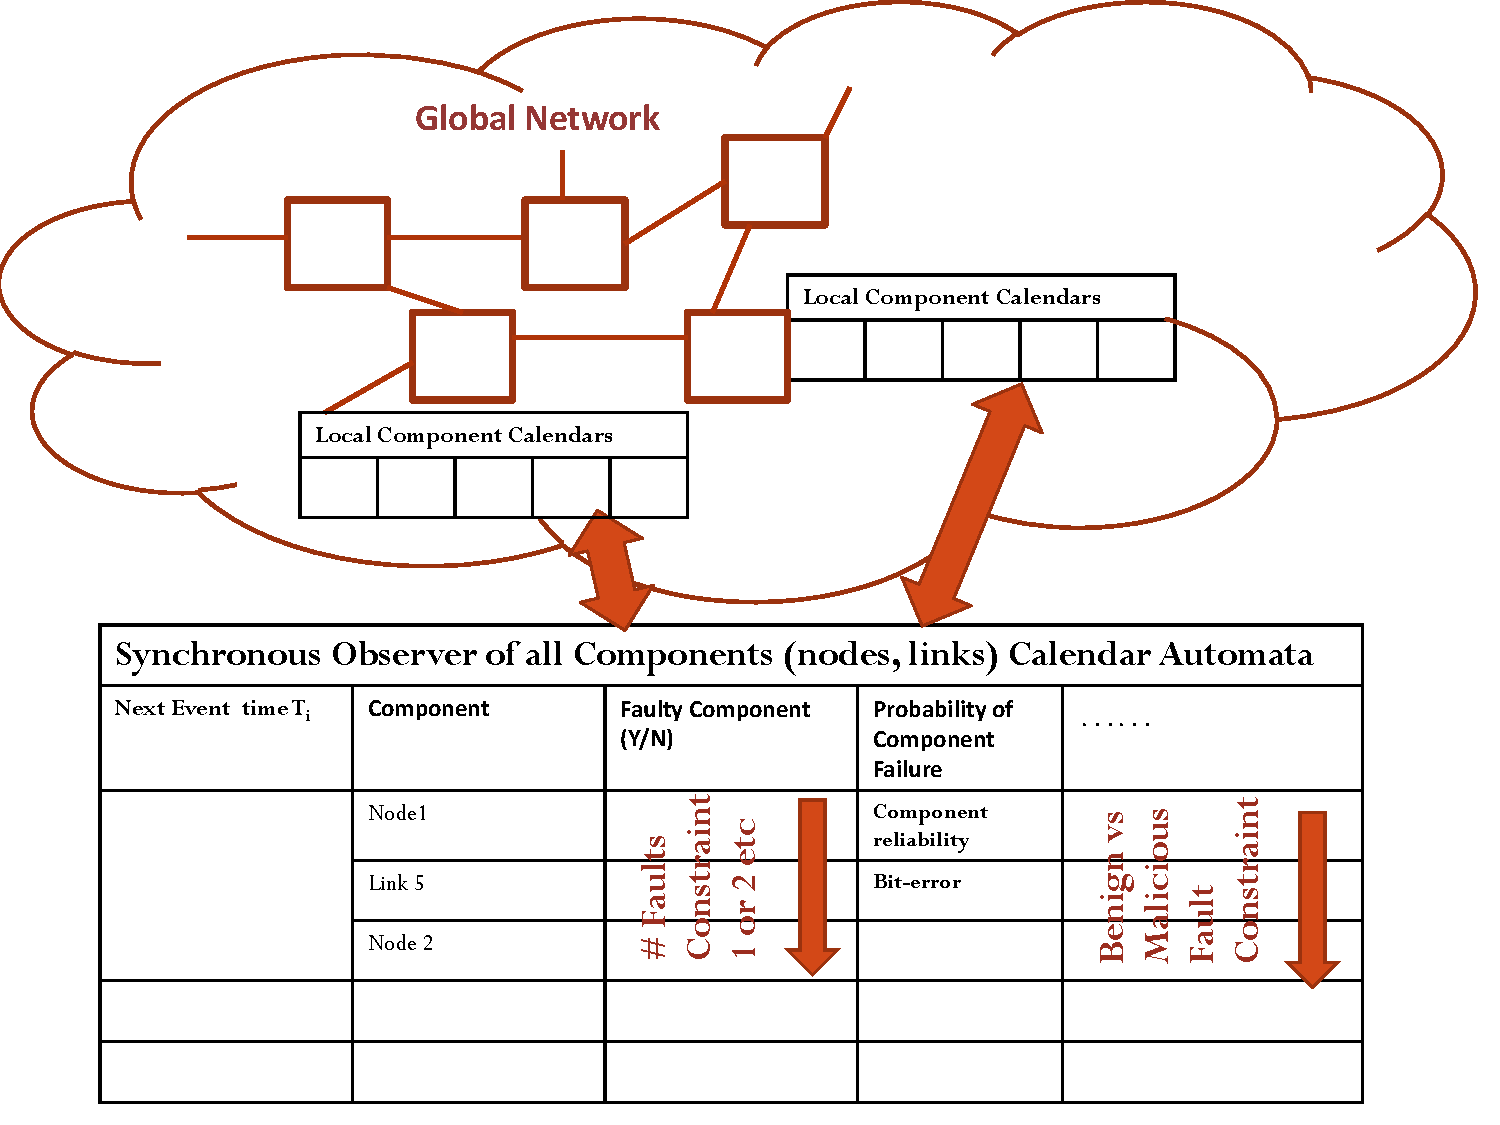
\includegraphics[width=0.7\textwidth]{figures/global_faults.pdf}
\caption{Global Fault Models}
\label{fig:global_faults}
\end{center}
\end{figure}

In Figure~\ref{fig:global_faults}, we use a single global calendar that acts as
a global fault ``bookkeeper'' interacting and constraining all local components'
calendar as well as constraining the global number of faults and all attributes
that need to managed at the system level, including components failure rates,
channel reliability etc.

Another issue that needs to addressed in the ADSL is a way to characterize fault
propagation through the networked system, originating in some component and
propagating from one component to another, as shown in the bottom of
Figure~\ref{fig:fault_propagation}. Faults introduced/propagated from upstream
components transforms to other faults based on protection mechanisms built into
each component (e.g., a commission fault transforms into an omission fault if a
bandwidth check is implemented as protection mechanism in a component).

To illustrate this in a concrete example, refer to a cyclic redundant check
(CRC) protection behavior illustrated at the top of
Figure~\ref{fig:fault_propagation}. Nominally in a fault-free operation,
$Node_1$ adds a CRC to a message when it transmits over the channel, and when
$Node_2$ receives the message, it does a CRC check by comparing the re-computed CRC
with the frame check sequence (FCS). If the check fails, the message is dropped, and if the check
passes, then the FCS is stripped and the message is forwarded. Note that fault-free
(nominal behavior) of a CRC check at the receiver is that (i) a good message is
never dropped incorrectly (ii) a bad (corrupt) message is dropped with high
probability and (iii) there is also a small finite probability that a bad
message escapes detection and drop (e.g. based on efficacy of CRC 32 etc)~\cite{crc}.

Value Fault~1 in Figure~\ref{fig:fault_propagation} introduced in the node
either at the indicated point or introduced upstream before that point and
propagated until that point will also continue to propagate downstream and CRC
offers no protection. This is because the FCS is added on an already corrupted
message. Value Fault~2 introduced in the channel will be protected by CRC
(modulo the CRC's efficacy). Value Fault~3 introduced in $Node_2$ at that point will
propagate downstream as it is after CRC protection.

The idea then is to capture a “fault transformation function” in every component
node/link based on behavior fault-protection schemes available at that component;
e.g., a value fault transforms to an omissive fault for CRC protection.  These will be
specified in a static manner at every component. This way, both horizontal
propagation of faults (CRC example) and vertical propagation of faults
(e.g., self-checking hardware) can be modeled as component “embedded” in another
component) can be captured in ADSL framework


\begin{figure}
\begin{center}
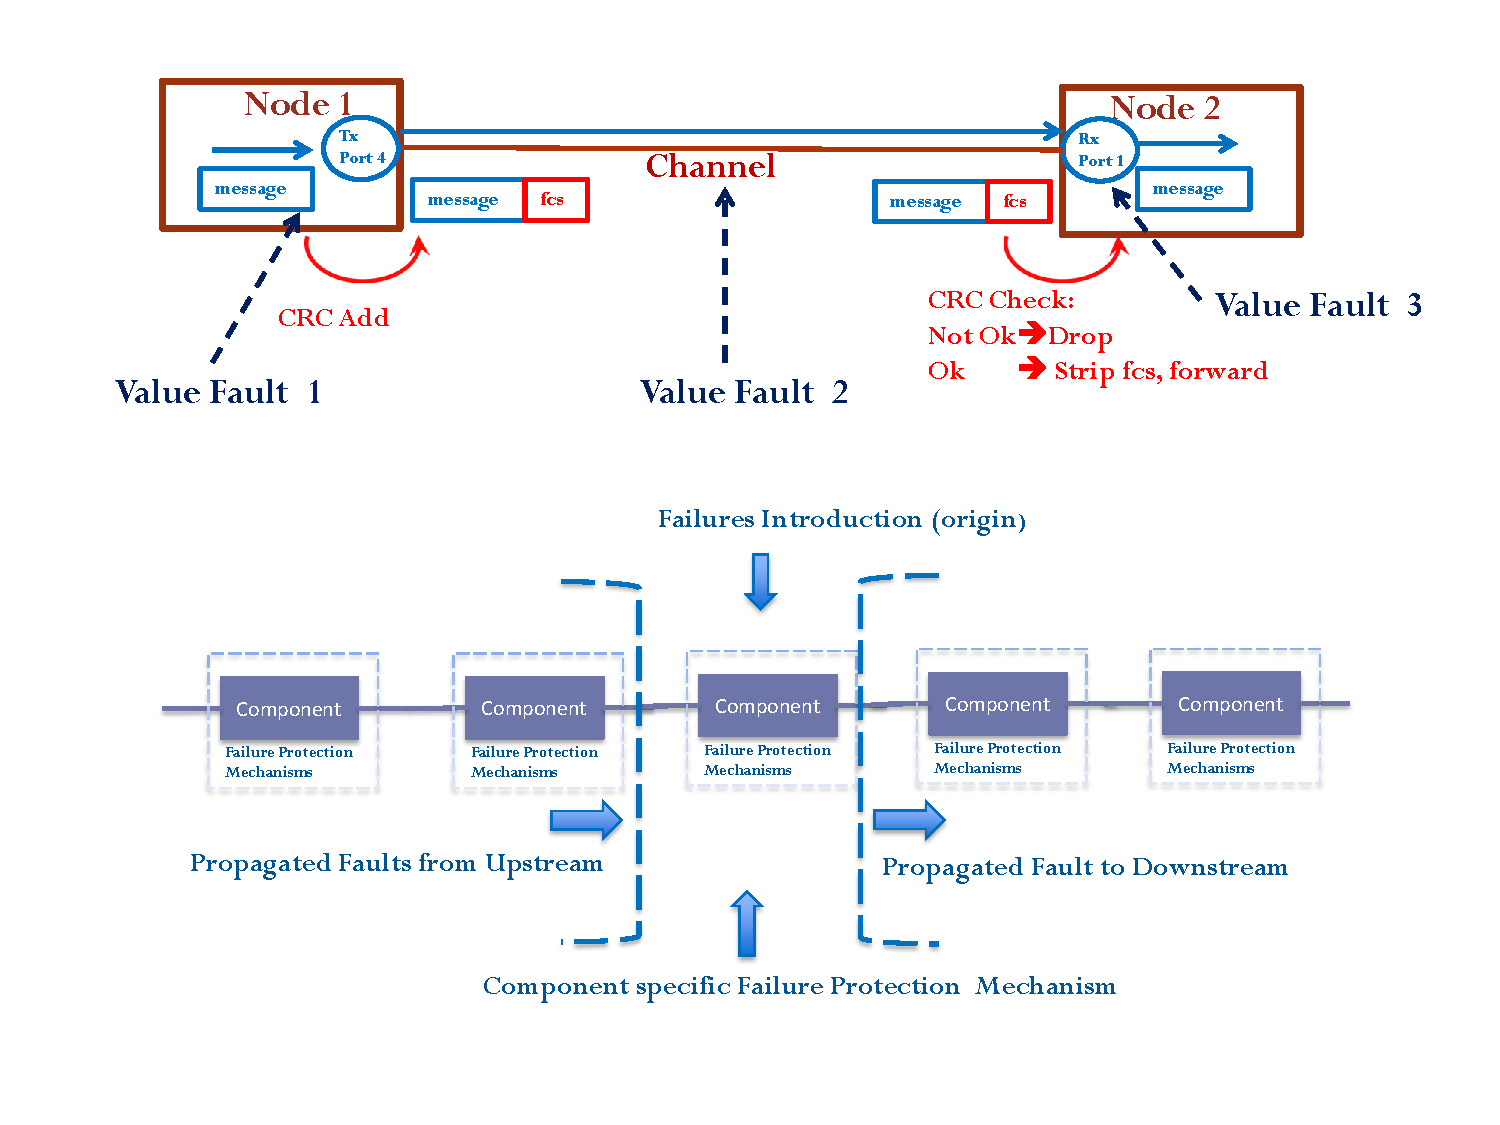
\includegraphics[width=0.7\textwidth]{figures/fault_propagation.pdf}
\caption{Fault Propagation}
\label{fig:fault_propagation}
\end{center}
\end{figure}
